%!TEX root = ../main.tex

\chapter{\texorpdfstring{Time distribution of \a\ events}{Time distribution of alpha-events}}%
\label{apdx:timealpha}

The time distribution of \Po\ decays is well known to be exponential, however, in the
presence of a \Pbl\ contamination a constant contribution can also be observed. \Pbl,
decaying to \Po, feeds a constant \Po\ component once their decay rates stabilize in a
secular equilibrium. To disentangle the two we fit the time distribution of events with
energies between 3.5~MeV and 5.25~MeV with a constant $C$ and an exponential function:
\[
  f(t) = C + N \exp\left( - \frac{\log2}{T_{1/2}}t \right)
\]
where $T_{1/2}=(138.4\pm0.2)$~days is the half-life of \Po. We use a Poisson likelihood
function corrected for data acquisition dead time~\cite{Cleveland1983} and model the time
bin content as follows
\[
  \nu_i = f_i^{\mathrm{LT}}
  \left\{ C \delta t + N \tau
    \left[
      \exp\left( -\frac{t_0 + i \delta t}{\tau} \right)  -
      \exp\left( -\frac{t_0 + (i+1) \delta t}{\tau} \right)
    \right]
  \right\}
\]
$C$ and $N$ are the amplitudes of the constant and the exponentially decaying components
and are the only two free fit parameters.  $f_i^{\mathrm{LT}}$ is the live-time fraction
in time-bin $i$ which is estimated from injected test pulser events, $\delta t$ is the
time-bin width and $\tau = T_{1/2} / \log2$.

The log-likelihood can be written as a sum:
\[
  \log \mathcal{L}_\alpha^\text{time}(C,N \,|\, n) =
  \sum_{i=1}^{N_\text{bins}} n_i \cdot
  \log\nu_i - \nu_i - \log n_i!
\]
We select only detectors that were ON or in anti-coincidence mode\footnote{Detectors in
anti-coincidence are not well energy-calibrated and generally discarded in data analysis.
Here, we are not interested in the precise energy of an event because the selected energy
window is large with respect to a possible miscalibration.} in the full data taking
period. In this way we avoid bias due to selection or deselection of particularly
contaminated detectors. Furthermore, we exclude the initial data-taking period between
December 2015 to January 2016 from the following analysis because of detector
instabilities after the \phasetwo\ upgrade works. The analyzed data span from
25$^\text{th}$ January 2016 to 3$^\text{rd}$ April 2018 and are split into two data sets
according to detector type, containing 27 \bege\ and 7 \scoax\ detectors. The fit results
are shown in \autoref{fig:apdx:timealpha:plotresults} and listed in
\cref{tab:apdx:timealpha:results}. For the \bege\ data set we find that about half of the
initial contamination decays exponentially while for the \scoax\ data set the ratio of $N$
to $C$ is about 5 to 1. After several \Po\ half-lives we expect a stable rate of
$\sim1~\alpha$/day in either data set.

\begin{figure}
  \centering
  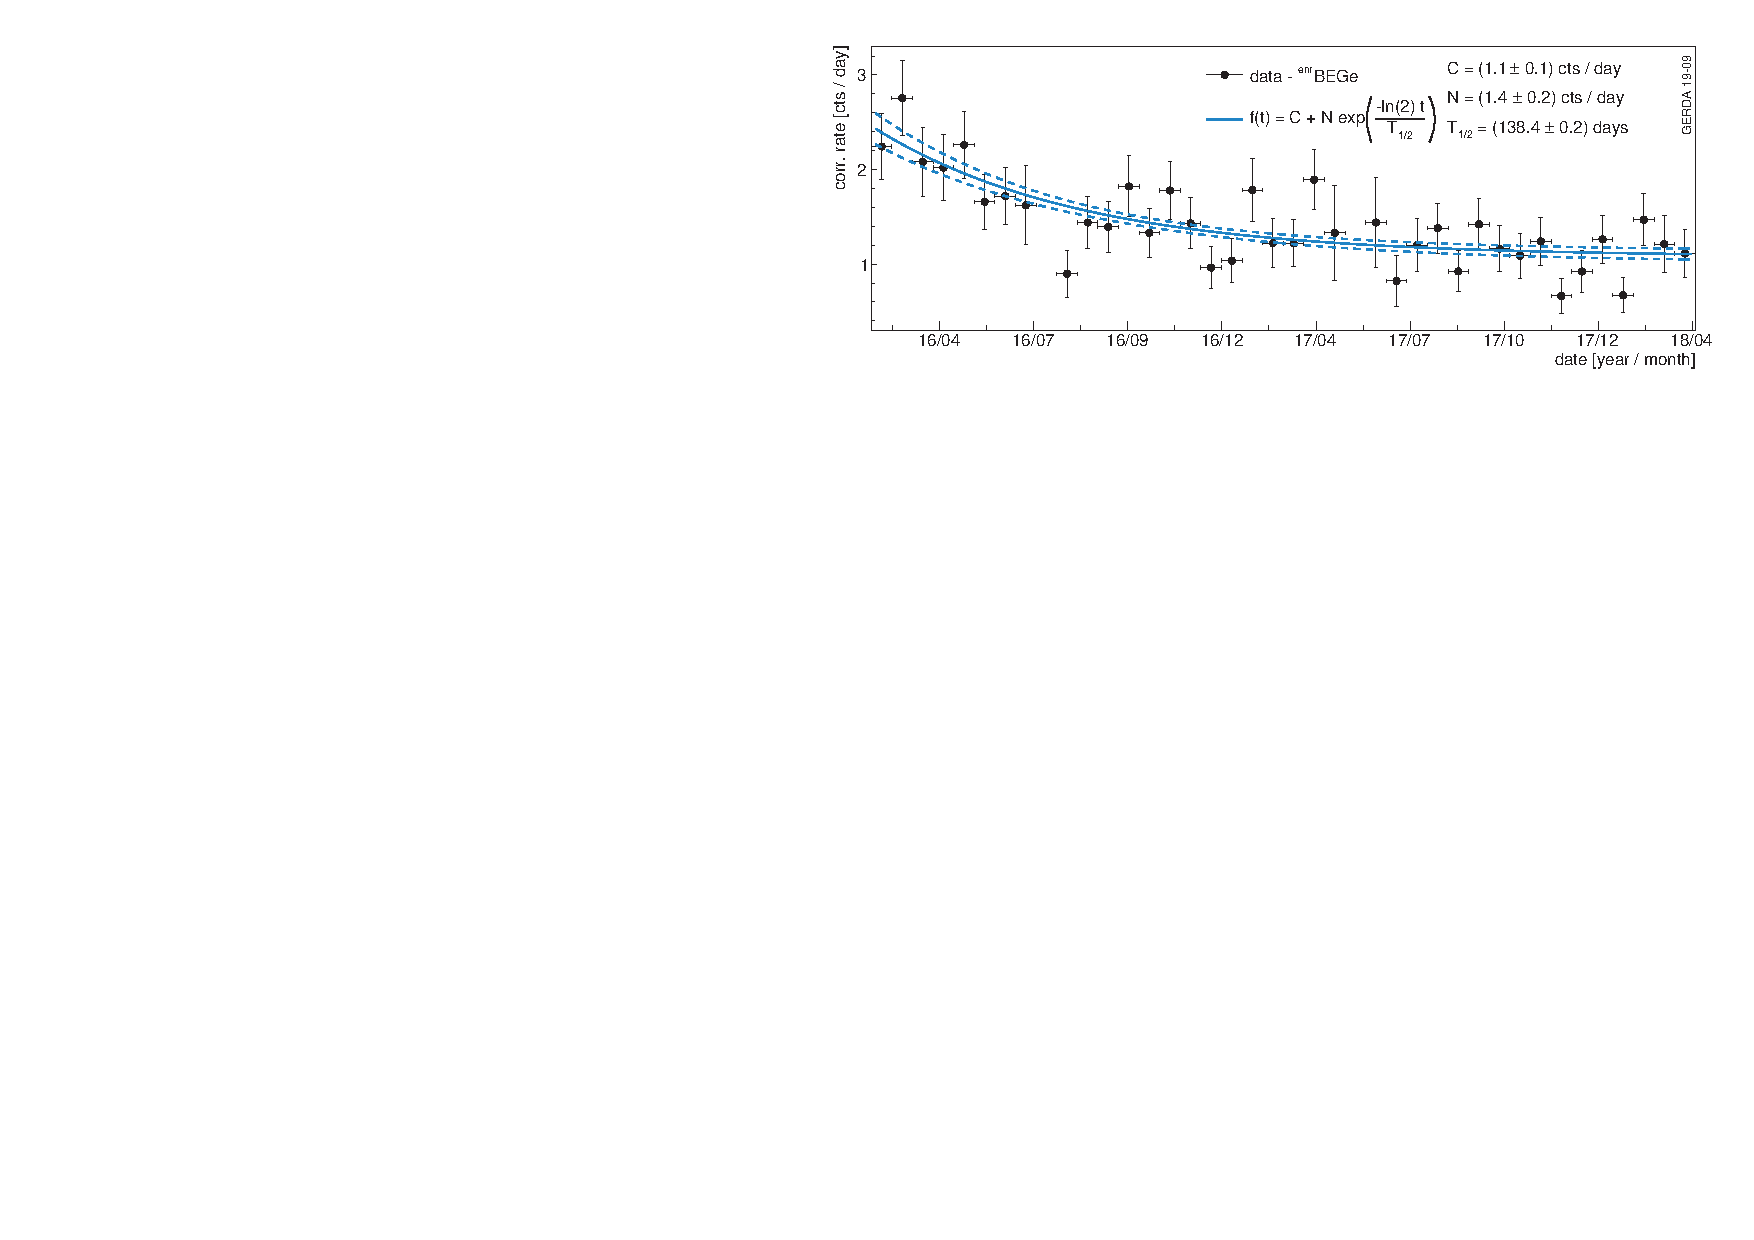
\includegraphics[width=0.8\textwidth]{plots/bkg/raw/ph2/results/amodel/timealpha-enrBEGe.pdf}
  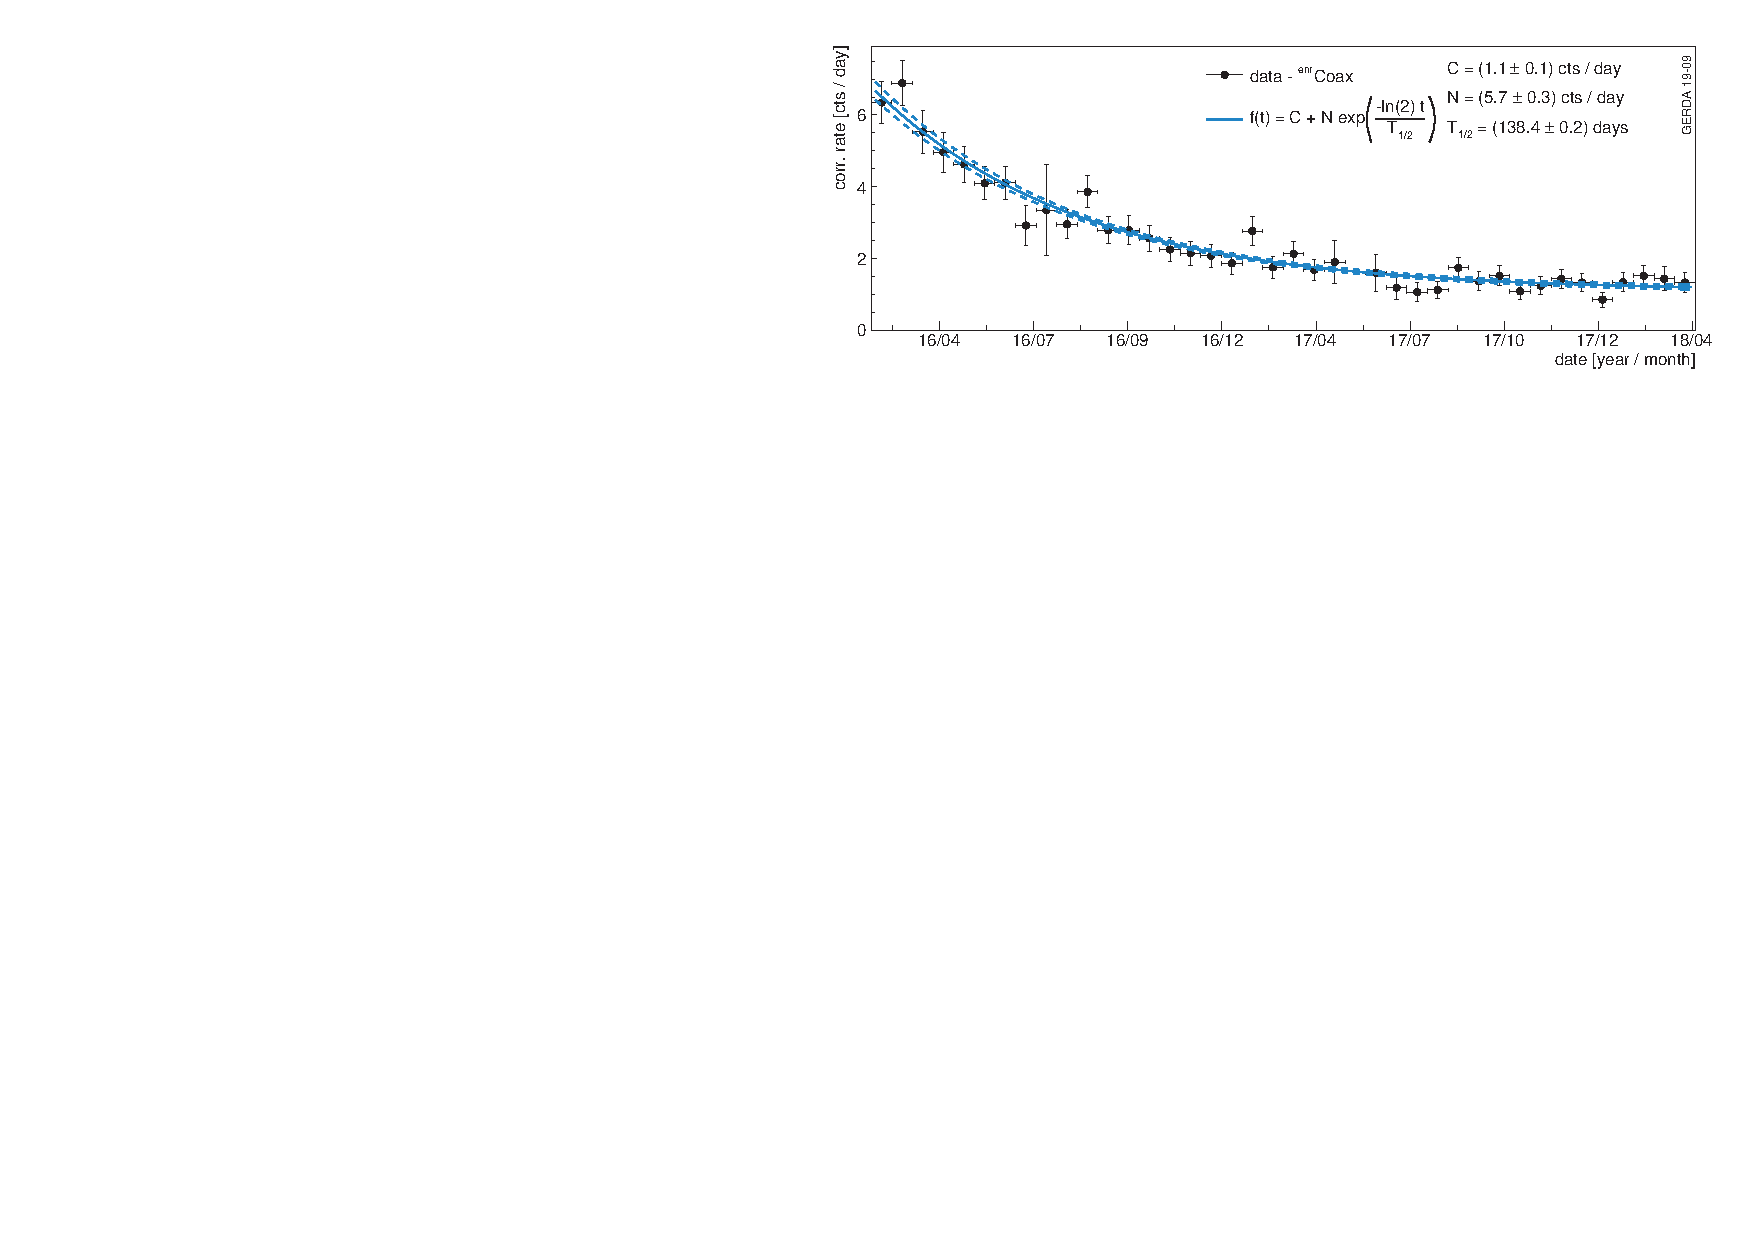
\includegraphics[width=0.8\textwidth]{plots/bkg/raw/ph2/results/amodel/timealpha-enrCoax.pdf}
  \caption{%
    \a\ events time distribution in $[3500,5250]$~keV with a binning of 20~days for 27
    \bege\ (top) and 7 \scoax\ (bottom) detectors.
  }\label{fig:apdx:timealpha:plotresults}
\end{figure}

\begin{table}
  \centering
  \caption{%
    Results of the \a\ events time distribution analysis in $[3500,5250]$~keV with a
    binning of 20~days for 27 \bege\ and 7 \scoax\ detectors.
  }\label{tab:apdx:timealpha:results}
  \addfontfeatures{Numbers=Tabular}
\begin{tabular}{cccccr@{ }l}
  \toprule
  \mr{2}{parameter} & \mr{2}{data} & \mr{2}{units}   & \mr{2}{global mode} & \mc{2}{marg.~mode}   \\
                    &              &                 &                     & \mc{2}{68\% C.I.}    \\
  \midrule
  \mr{2}{$C$}       & \bege\       & \mr{2}{cts/day} & $1.06$              & 1.05 & $[1.00,1.12]$ \\
                    & \scoax\      &                 & $1.09$              & 1.09 & $[1.02,1.16]$ \\
  \midrule
  \mr{2}{$N$}       & \bege\       & \mr{2}{cts/day} & $1.32$              & 1.33 & $[1.13,1.53]$ \\
                    & \scoax\      &                 & $5.71$              & 5.70 & $[5.42,6.01]$ \\
  \bottomrule
\end{tabular}

\end{table}

% vim: tw=90
